\documentclass[a4paper, 12pt]{article}
\setlength{\parindent}{0em}

\usepackage{amssymb}
\usepackage{amsmath}
\usepackage[document]{ragged2e}
\usepackage{comment}
\usepackage{upgreek}
\usepackage{gb4e}
\noautomath
\usepackage{multicol}
\usepackage{tipa}
\usepackage{longtable}
\usepackage{qtree}
\usepackage{tikz-qtree}
\usepackage{textcomp}
\usepackage{hyperref}
\usepackage{graphicx}
\usepackage{hyperref}
\usepackage{float}

\usepackage{pifont}
\usepackage[mathscr]{eucal}
\usepackage[margin=1in]{geometry}
\newcommand{\xmark}{\ding{55}}%5
%\pagenumbering{gobble}

\def\HS{\space\space}

\setlength{\LTleft}{0pt}

\title{Indonesian Phonetics}
\date{}
\author{Ryan Sie \\ LIGN 110}


\begin{document}
\maketitle


\section{Bahasa Indonesia}

Indonesian, known as Bahasa Indonesia to its speakers, is the official language of Indonesia today, with approximately 43 million native speakers, and about 156 million more who speak it as a second language (Indonesia Census 2010). It is a very close relative to Malay within the Austronesian language family. Outside of Indonesia, Indonesian is spoken abroad by people of Indonesian background in countries such as the United States, the Netherlands, and Singapore.
\bigskip

My consultant for this project is Guido Sie, a native Indonesian speaker who grew up in Surabaya, Indonesia. In addition to Indonesian, he also speaks English, and is familiar with Dutch and Javanese from his experiences growing up in Surabaya. He has been living in the United States for over 35 years now, though still uses Indonesian to converse with friends and family periodically. Indonesian orthography uses the roman alphabet like English, and Guido is able to read Indonesian clearly. 
\bigskip

The primary source of outside knowledge used to supplement this report is the journal article \textit{Indonesian} by Craig Soderberg and Kenneth Olson. This article covers the phonetics of Indonesian, and was published in \textit{Journal of the International Phonetic Association: Illustrations of the IPA} in 2008. I used both examples from this article, as well as other words that Guido and I agreed on.

\section{Consonants}

There are a total of 22 consonant phonemes in Indonesian, shown below. 

\begin{center}
\noindent\makebox[\textwidth]{%
	\begin{tabular}{|p{2.15cm}|*{8}{c |}}
	\hline
	 & Bilabial & Labio-dental & Dental & Alveolar & Post-Alveolar & Palatal & Velar & Glottal \\ \hline
	Stop & p\HS b &  & \textsubbridge{t} &  d &  & & k g & \textipa{P}  \\ \hline
	Affricate & & & & & \textteshlig \HS \textdyoghlig & & & \\ \hline
	Fricative & & f & & s z & \textipa{S} & & & h \\ \hline
	Nasal & m & & & n & & \textltailn & \textipa{N} & \\ \hline
	Flap/Trill & & & & r & & & & \\ \hline
	Approximant & w & & & & & j & & \\ \hline
	Lateral Approximant & & & & l & & & & \\ \hline	
	\end{tabular}	
}
\end{center}

\bigskip

It is interesting to note that every consonant in Indonesian appears as a separate phoneme. While there are an abundance of consonant allophones, each one also appears in other contexts as their own phonemes. As we will discuss later however, this is not the case with vowels.

\bigskip

Below is a list of Indonesian words demonstrating these different phonemes. The examples are provided in the same order as in the given recording. Each word is given via IPA transcription (broad form is included if different than narrow form), Indonesian orthography, and an English translation. Most consonants are demonstrated word-initially preceding the vowel /a/.  

\bigskip

The first group shows the bilabial and labio-dental sounds: /p/, /b/, /m/, /w/, /f/:  

\begin{longtable}[l]{lp{2cm}lp{2cm}}

\hypertarget{paling}{1.} \textipa{["pal{\textsci}N]} /\textipa{paliN}/ & \textit{paling} &	 'most' \\

2. \textipa{["bali]} & \textit{Bali} & (name of an island) \\

3. \textipa{["malu]} & \textit{malu} & 'ashamed' \\

4. \textipa{["wali]} & \textit{wali} & 'guardian' \\

\hypertarget{fakta}{5.} \textipa{["fak\textcorner\|[ta]} & \textit{fakta} & 'fact' \\

\end{longtable}

\medskip

The next group illustrates the alveolar and post-alveolar fricatives /z/, /s/, /\textesh/, as well as the two alveolar liquids /r/, and /l/:

\begin{longtable}[l]{lp{2cm}lp{2cm}}

\hypertarget{zat}{6.} \textipa{["za\|[t\textcorner]} & \textit{zat} & 'substance' \\

\hypertarget{sabuk}{7.} \textipa{[sa"b{\textupsilon}P]} /\textipa{sabuk}/ & \textit{sabuk} & 'belt, sash' \\

8. \textipa{["Saban]} & \textit{syaban} & 'Sha'ban, 8th month of the Islamic calendar' \\

\hypertarget{rabu}{9.} \textipa{[ra"bu]} & \textit{rabu} & 'Wednesday' \\

10. \textipa{["labu]} & \textit{labu} & 'squash, gourd' \\

\end{longtable}

\medskip

The next group of words demonstrates the post-alveolar affricates /\textteshlig/ and /\textdyoghlig/, as well as the denti-alveolar/alveolar stops /\textipa{\|[t}/ and /d/.


\begin{longtable}[l]{lp{2cm}lp{2cm}}

11. \textipa{["{\textteshlig}ari]} & \textit{cari} & 'find' \\

12. \textipa{["{\textdyoghlig}ari]} & \textit{jari} & 'finger' \\

13. \textipa{["\|[tari]} & \textit{tari} & 'dance' \\

14. \textipa{["dari]} & \textit{dari} & 'from'	\\
	
\end{longtable}

\bigskip

The following words consist of the remaining nasal phonemes /n/, /\textltailn/, and /\textipa{N}/: 

\begin{longtable}[l]{lp{2cm}lp{2cm}}
	
15. \textipa{[na"rasi]} & \textit{narasi} & 'narrative' \\

\hypertarget{nyaris}{16.} \textipa{["{\textltailn}ar{\textsci}s]} /\textipa{{\textltailn}aris}/ & \textit{nyaris} & 'almost' \\

\hypertarget{ngantuk}{17.} \textipa{[Nan"\|[t{\textupsilon}P]} /\textipa{Nan\|[tuP}/ & \textit{ngantuk} & 'sleepy' \\
	
\end{longtable}

\medskip

The next group shows the palatal approximant /j/, and the velar stops /k/ and /g/:

\begin{longtable}[l]{lp{2cm}lp{2cm}}

18. \textipa{["jaN]} & \textit{yang} & 'that, which' \\

\hypertarget{kantong}{19.} \textipa{["kan\|[t{\textopeno}N]} /\textipa{kan\|[toN}/ & \textit{kantong} & 'bag' \\

\hypertarget{gantung}{20.} \textipa{["gan\|[toN]} /\textipa{gan\|[tuN}/ & \textit{gantung} & 'hanging' \\
	
\end{longtable}

\bigskip

Lastly we compare the two glottal consonants /\textipa{P}/ and /h/. Because /\textipa{P}/ does not appear word initially as a phoneme, we frame both consonants between two /a/ vowels:

\bigskip

\begin{longtable}[l]{lp{2cm}lp{2cm}}
	

21. \textipa{["maPaf]} & \textit{ma'af} & 'sorry' \\

22. \textipa{["paha]} & \textit{paha} & 'thigh'	\\
	
\end{longtable}

According to Soderberg and Olson, /\textglotstop/ appears as a phoneme exclusively between two vowels in three situations. It may appear in words like in (21), found most often in words of Arabic origin. It may also appear between a affixes and stems which meet at vowel boundaries.

\medskip

\section{Vowels}

There are a total of 6 vowel phonemes in Indonesian, shown below, with 4 additional vowel allophones shown in parentheses.
\begin{center}
	\begin{tabular}{|p{2cm}|*{3}{c |}}
		\hline
		& Front & Central & Back \\ \hline
		High & i & & u \\ \hline
		High-mid  & (\textsci) & & (\textupsilon) \\ 
		& e &  & o\\ \hline
		Mid & & \textschwa & \\ \hline
		Low-mid  & (\textepsilon) & & (\textopeno) \\ \hline
		Low &  & a & \\ \hline
	\end{tabular}	\\
\end{center}

Below are words illustrating the six separate vowel phonemes. The first four show contrasts between /i/, /a/, /u/, and /o/. Each vowel in this group is framed between /b/ and /r/.

\begin{longtable}[l]{lp{2cm}lp{2cm}}

23. \textipa{["biru]} & \textit{biru} & 'blue' \\

24. \textipa{["baru]} & \textit{baru} & 'new' \\

\hypertarget{buruk}{25.} \textipa{[bu"ruP]} & \textit{buruk} & 'bad, poor' \\

\hypertarget{borobudur}{26.} \textipa{[""boro"budur]} & \textit{Borobudur} & (name of a temple in Central Java)

\end{longtable}

\bigskip

The next pair compares the remaining two vowel phonemes /e/ and /\textschwa/, using the frame /b?b/:

\begin{longtable}[l]{lp{2cm}lp{2cm}}

27. \textipa{["bebas]} & \textit{bebas} & 'free' \\

28. \textipa{[b@"brapa]} & \textit{beberapa} & 'several' \\

\end{longtable}

\medskip

\section{Allophones}

As mentioned previously, the various consonant allophones in Indonesian all appear as separate phonemes themselves. However, some consonants have features still worth discussing, which have already appeared in the words above. For instance, the voiceless stops /p/, /\textipa{\|[t}/, and /k/ are all produced unaspirated. In addition, all are unreleased in syllable final position, as seen in \hyperlink{fakta}{(5) - \textit{fakta}} - \textipa{["fak\textcorner\|[ta]} and \hyperlink{zat}{(6) - \textit{zat}} -   \textipa{["za\|[t\textcorner]}. In fact, in some words, syllable final /k/ was realized as [\textglotstop]. This behavior can be seen above in the words \hyperlink{sabuk}{(7) - \textit{sabuk}} - \textipa{[sa"b{\textupsilon}P]} and \hyperlink{ngantuk}{(17) - \textit{ngantuk}} - \textipa{[Nan"\|[t{\textupsilon}P]}. According to Soderberg and Olson, this behavior occurs only in non-loanwords, which explains why the change was not present in \textipa{["fak\textcorner\|[ta]}. There are many other interesting consonant allophones, but the rest of the section will be devoted to discussing vowels, which consist of entirely new sounds.

\bigskip

The 4 vowels [\textsci], [\textepsilon], [\textupsilon], and  [\textopeno] appear as allophones in Indonesian of /i/, /e/, /u/, and /o/, respectively. They are typically lowered in a final closed syllable, or in a penultimate syllable which is followed by a final closed syllable whose vowel agrees in height (Soderberg and Olson, 2008). Guido seemed to closely follow this pattern throughout the recording. \\

\bigskip

To demonstrate, here is a pair of words demonstrating [\textepsilon] as an allophone of /e/:

\begin{longtable}[l]{lp{2cm}lp{4cm}}
	
29. /sepele/ & \textipa{[s@"pele]} & \textit{sepele} & 'not important' \\
\hypertarget{oleh}{30.} /oleh/ & \textipa{[o"lEh]} & \textit{oleh} & 'by' \\	
	
\end{longtable}

In \textipa{[s@"pele]}, the open final syllable /le/ is produced with an unchanged [e]. In \textipa{[o"lEh]} however, the presence of the /h/ in the closed final syllable /leh/ results in /e/ being lowered to [\textepsilon]. In addition, although /e/ matches /o/ in height, we see that the initial /o/ is \textit{not} lowered to [\textopeno]. \\

\bigskip

Similarly, the next pair illustrates [\textopeno] as an allophone of /o/:

\begin{longtable}[l]{lp{2cm}lp{4cm}}
	
31. /\textipa{\|[t}oko/ & \textipa{["\|[toko]} & \textit{toko} & 'store' \\

\hypertarget{tokoh}{32.} /\textipa{\|[t}okoh/ & \textipa{[\|[tO"kOh]} & \textit{tokoh} & 'figure, character' \\
	
\end{longtable}

As before, the open final syllable /ko/ in \textipa{["\|[toko]} is produced with an unchanged [o] vowel. On the other hand, the closed final syllable /koh/ in \textipa{[\|[tO"kOh]} is produced with the lowered [\textopeno]. In addition, this time we also see that in the penultimate syllable /\textipa{\|[t}o/ in \textipa{[\|[tO"kOh]}, the /o/ is also lowered to [\textopeno], since /o/ agrees in height with itself. Meanwhile the /o/ in the penultimate syllable /\textipa{\|[t}o/ of \textipa{["\|[toko]} remains unchanged, since the following /ko/ is not closed.

\bigskip

The fact that the first pair of words spoken by Guido did not follow the penultimate vowel-height rule suggests that this specific rule may be less prominent in his dialect. More discussion of this appears later on in final section of this report - Section 6, the \hyperlink{sentence}{sentence}.

\bigskip

An example of [\textsci] as an allophone of /i/ can be seen in \hyperlink{paling}{(1) - \textit{paling}} - \textipa{["pal{\textsci}N]} and \hyperlink{nyaris}{(16) - \textit{nyaris}} - [\textipa{{\textltailn}ar{\textsci}s}]. Similarly, evidence of [\textupsilon] as an allophone of /u/ is present in \hyperlink{sabuk}{(7) - \textit{sabuk}} - \textipa{[sa"b{\textupsilon}P]} and \hyperlink{ngantuk}{(17) - \textit{ngantuk}} - \textipa{[Nan"\|[t{\textupsilon}P]}. 

\bigskip

One behavior displayed that is worth noting is that /u/ was not always realized as [\textupsilon] in a final closed syllable. For example, in \hyperlink{buruk}{(25) - \textit{buruk}} - \textipa{[bu"ruP]}, and \hyperlink{borobudur}{(26) - \textit{borobudur}} - \textipa{[""boro"budur]}, the /u/ in the final closed syllable remained unchanged. On another note, it appeared that in some contexts, /u/ in a final closed syllable was lowered to /o/. For instance, in \hyperlink{gantung}{(20) - \textit{gantung}} - /gan\textipa{\|[t}u\textipa{N}/ - \textipa{["gan\|[toN]}, /u/ is realized as [o]. Now one might argue that perhaps /o/ is the actually phoneme present for this specific word. However, if this were the case, we would have expected it to lower to [\textopeno], since it appears in a final closed syllable. In fact, in the preceding word \hyperlink{kantong}{(19) - \textit{kantong}} - /kan\textipa{\|[t}o\textipa{N}/ - \textipa{["kan\|[tON]}, the final syllable \textipa{/\|[toN/} is realized as \textipa{[\|[tON]}. So if the vowel phoneme in the final syllable of \textipa{["gan\|[toN]} was really /o/, we would expect its behavior to mirror the \textipa{/\|[toN/} to \textipa{[\|[tON]} change. Since it does not, then it seems more likely that we are actually seeing the phoneme /u/ being lowered to [o]. This behavior is again seen in words (34) and (35) in the next section.

\bigskip

Similarly, Guido sometimes produced /a/ with a different vowel quality for certain words. After checking the formant listings of a sample of 7 words containing /a/, here is what I found: \\

\begin{figure}[H]
	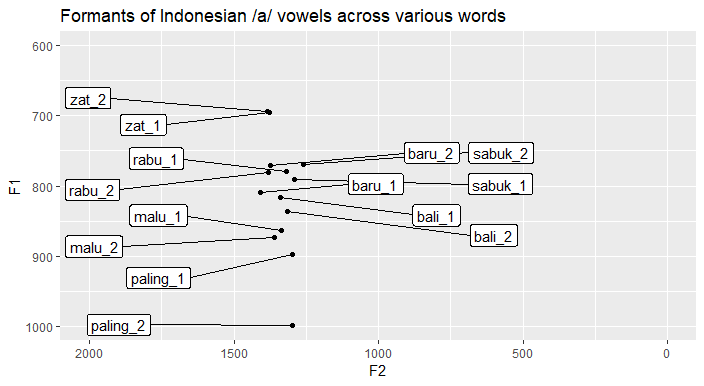
\includegraphics[width=\linewidth]{images/a_formants.png}
	\caption{F1 and F2 listings of /a/ vowels across various words}
	\label{fig:a_formants} 
\end{figure}
\medskip

Figure 1 shows that /a/ is most often produced with F1 around 800 and F2 around 1300. However, in some contexts, the F1 seems to differ significantly. In particular, \hyperlink{zat}{(6) - \textit{zat}} - \textipa{["za\|[t\textcorner]} - 'substance', seems to show a lower than typical F1, being produced with a higher /a/. On the other hand, \hyperlink{paling}{(1) - \textit{paling}} - \textipa{["pal{\textsci}N]} - 'most', seems to have a higher F1 than usual, being produced with a lower /a/. One theory I had initially was perhaps it had something to do with the fact that \textipa{["za\|[t\textcorner]} is a word of Arabic origin. However, checking the formants for another word of Arabic origin, (22) - \textipa{["maPaf]} showed F1 - 860, F2 - 1250, which is around the average. Thus, there does not seem to be any obvious systematic pattern to why these /a/ formants differ.

\bigskip

\section{Stress}

According to Soderberg and Olson, the primary stress in unaffixed Indonesian words typically appears on the penultimate syllable. The primary exception to this rule is if the penultimate syllable contains /\textschwa/. In this case, the stress will most often move to the final syllable, though some dialects may move it to the previous syllable in certain contexts.  In addition, stress does not display any phonemic contrast in Indonesian.

\medskip

Below are a few examples demonstrating how Guido applied stress in the absence and presence of a /\textschwa/ in the penultimate syllable.

\medskip

\begin{longtable}[l]{lp{2cm}lp{4cm}}
	
33. /pin\textipa{\|[t}u/ & \textipa{["pin\|[tu]} & \textit{pintu} & 'door' \\

34. /p{\textschwa}ru\textipa{\|[t}/ & \textipa{[p@"ro\|[t\textcorner]} & \textit{perut} & 'stomach \\

35. /s{\textschwa}b{\textschwa}lum/ & \textipa{[""s@b@"lom]} & \textit{sebelum} & 'before'	
	
\end{longtable}

While he did demonstrate the penultimate to ultimate stress change with the presence of /\textschwa/in the penultimate syllable, he also applied the change in other contexts where the vowel in the penultimate syllable differed.

\bigskip

For instance, in the some of the preceding words he moved the stress to the final syllable, though the vowel in the penultimate syllable was /a/: \hyperlink{sabuk}{(7) - \textit{sabuk}} - \textipa{[sa"b{\textupsilon}P]} - 'belt, sash'; \hyperlink{rabu}{(9) \textit{rabu}} - \textipa{[ra"bu]} - 'Wednesday'; and \hyperlink{ngantuk}{(17) - \textit{ngantuk}} - \textipa{[Nan"\|[t{\textupsilon}P]} - 'sleepy';

\medskip

Similarly, in \hyperlink{buruk}{(25) - \textit{buruk}} - \textipa{[bu"ruP]} - 'bad, poor', stress changes to the ultimate syllable following /u/, and in \hyperlink{oleh}{(30) - \textit{oleh}} - \textipa{[o"lEh]} - 'by' and \hyperlink{tokoh}{(32) - \textit{tokoh}} - \textipa{[\|[tO"kOh]} - 'figure, character', stress changes to the ultimate syllable following /o/.\\

\bigskip

Upon asking him about this behavior, he said that it was just the natural way he has always said those words. As a result, the most likely explanation is that it is simply a feature of the dialect of Indonesian he grew up speaking in Surabaya. In particular, perhaps it has something to do with the coda of the final syllable. One pattern I noticed among the words discussed above is that 5 out of the 6 ended in one of the two glottal consonants - /\textipa{P}/ or /h/. However, more data and research would be needed to test the hypothesis.

\section{Sentence}

\hypertarget{sentence}{Below} is a short sentence in Indonesian demonstrating a couple of the words above in a single utterance. It is provided in broad and narrow IPA, as well as a gloss and in Indonesian orthography.

\begin{longtable}[l]{lp{2cm} lp{2cm} lp{2cm}}

/\textipa{toloN} & \textipa{buku} & \textipa{jaN} & \textipa{biru} & \textipa{dibuNkus}/ \\
	
[\textipa{"\|[tolON} & \textipa{"buku} & \textipa{"jaN} & \textipa{"biru} & \textipa{di"buNk{\textupsilon}s}] \\

please & book & that (is) & blue & passive-wrap \\

Tolong & buku & yang & biru & dibungkus. \\

\end{longtable}


"Please wrap the blue book". \\

\medskip

Again we see the allophones [\textipa{O}] and [\textupsilon] in the final closed syllables of [\textipa{"tolON}] and \textipa{[di"buNk{\textupsilon}s]}, respectively. Note that the /o/ in the penultimate syllable /to/ remains unchanged in [\textipa{"tolON}]. Similarly, the /u/ of the penultimate syllable /bu\textipa{N}/ in [\textipa{di"buNk{\textupsilon}s}] remains unchanged, even though /u/ agrees with itself in height. This acts as more evidence that the penultimate vowel-height allophone rule change is not as prominent in the dialect of Indonesian Guido speaks.

\section{References}

Indonesia Population Census (2010), available at \\ \href{https://web.archive.org/web/20150402221528/http://www.bps.go.id/index.php/publikasi/14}{https://web.archive.org/web/20150402221528/http://www.bps.go.id/index.php/publikasi/14} 
\medskip

“Indonesian.” Ethnologue, \href{www.ethnologue.com/language/ind}{https://www.ethnologue.com/language/ind}.
\bigskip

Soderberg, Craig D., and Kenneth S. Olson. “Indonesian.” Journal of the International Phonetic Association, vol. 38, no. 02, 2008, doi:10.1017/s0025100308003320.
\bigskip

	
\end{document}
	